\section{Backup}

\begin{frame}{OpenFOAM Overview}
\begin{itemize}
\item Open-source, free, computational fluid dynamics toolbox 
\item Written in C++, has many solvers 
\item No GUI, file-based input and control
\end{itemize}
\end{frame}

\begin{frame}[allowframebreaks]{Governing Equations}
Total energy \cite{kuo} can be written as 
\begin{equation}
E = h - \frac{p}{\rho} +\frac{1}{2} \left(\bm{u}\cdot\bm{u}\right)\,,
\end{equation}
where the total summed enthalpy is written \cite{kuo} as 
\begin{equation}
h = \sum_{i = 1}^Nh_{s,i}Y_i\,,
\end{equation}
and the species total enthalpy \cite{kuo} is given by 
\begin{equation}
h_{i} = \Delta h_{f,i}^0 + h_{s,i}\,,
\end{equation}
with the sensible enthalpy for the $i$th species expressed as
\begin{equation}
h_{s,i} = \int_{T_0}^T C_{p,i}\mathrm{d}T\,,
\end{equation}
Here $C_{p,i}$ is the specific heat for the $i$th species, $T$ is the temperature, and $T_0$ is an initial, or reference, temperature. The equation of state is expressed as 
\begin{equation}
p = \rho R T\,,
\end{equation}
where $R=R_u/W$. Specific heat $C_{p,i}=C_{p,i}(T)$ from NIST JANAF \cite{janaf} lookup tables.  
\end{frame}


\subsection{OpenFOAM Numerical Setup}

\begin{frame}{OpenFOAM Finite Volume Numerical Schemes}
\begin{table}[t!]
\centering
%\caption{OpenFOAM finite volume numerical schemes applied during solving}
%\label{tab:numschemes}
\scalebox{0.9}{
\begin{tabular}{ccc}
Term & OpenFOAM Variable & Numerical Scheme \\ \hline 
Flux Scheme & \texttt{fluxScheme} & Kurganov \\ 
Time Scheme & \texttt{ddtSchemes} & Euler \\
Gradient Schemes & \texttt{gradSchemes} & Gauss linear \\ 
Divergence Schemes & \texttt{divSchemes} & none by default \\ 
& \texttt{div(tauMC)} & linear \\ 
& \texttt{div(phi,}specie\texttt{)} & van Leer \\ 
Laplacian Schemes & \texttt{laplacianSchemes} & Gauss linear uncorrected \\ 
Interpolation Schemes & \texttt{interpolationSchemes} & default linear \\
& \texttt{reconstruct(rho)} & Minmod \\ 
& \texttt{reconstruct(U)} & MinmodV \\ 
& \texttt{reconstruct(T)} & Minmod \\ 
& \texttt{reconstruct(Yi)} & Minmod \\ 
Surface Normal Gradient Schemes & \texttt{snGradSchemes} & uncorrected \\
\end{tabular}
}
\end{table}
\end{frame}

\begin{frame}{OpenFOAM Finite Volume Numerical Solvers}
\begin{table}[t!]
\centering
%\caption{Finite volume numerical solvers and preconditioners used for solution variables}
%\label{tab:numerics}
\begin{tabular}{cccc}
Variable & Solver & Parameter & Value \\ \hline 
\texttt{e}, \texttt{Y} & \texttt{PBiCGStab} & Preconditioner & \texttt{DILU} \\ 
& & Tolerance & \texttt{1e-17} \\ 
& & Relative tolerance & 0 \\\hline
\texttt{U} & \texttt{PBiCGStab} & Preconditioner & \texttt{DIC} \\ 
& & Tolerance & \texttt{1e-15} \\ 
& & Relative tolerance & 0 \\\hline
\texttt{rho} & \texttt{diagonal} & & \\
\end{tabular}
\end{table}
\end{frame}

\subsection{OpenFOAM Case Setup}

\begin{frame}{OpenFOAM Directory Structure}
An OpenFOAM case is divided into:
\begin{itemize}
\item \texttt{0/}: holds initial conditions and boundary conditions for quantities like pressure, temperature, velocity, etc. 
\item \texttt{constant/}: holds thermophysical quantities and some mesh information 
\item \texttt{system/}: contains numerical settings, mesh setup, and simulation settings
\end{itemize}
\end{frame}

\begin{frame}{OpenFOAM \texttt{constant/} Directory}
Contains:
\begin{itemize}
\item \texttt{chemistryProperties}
\item \texttt{combustionProperties}
\item \texttt{dynamicMeshDict}
\item \texttt{reactions}
\item \texttt{thermo.compressibleGas}
\item \texttt{thermophysicalProperties}
\item \texttt{turbulenceProperties}
\end{itemize}
\end{frame}

\begin{frame}{OpenFOAM \texttt{system/} Directory}
Contains:
\begin{itemize}
\item \texttt{blockMeshDict}
\item \texttt{controlDict}
\item \texttt{decomposeParDict}
\item \texttt{setFieldsDict}/\texttt{funkySetFieldsDict}
\item \texttt{fvSchemes}
\item \texttt{fvSolution}
\item files defining post-processing line sampling
\end{itemize}
\end{frame}

\subsection{Arrhenius Pre-exponential Factor Sweep}
\begin{frame}{Arrhenius Pre-exponential Factor Sweep, Refined: Pressure Distribution}
\begin{figure}
\centering
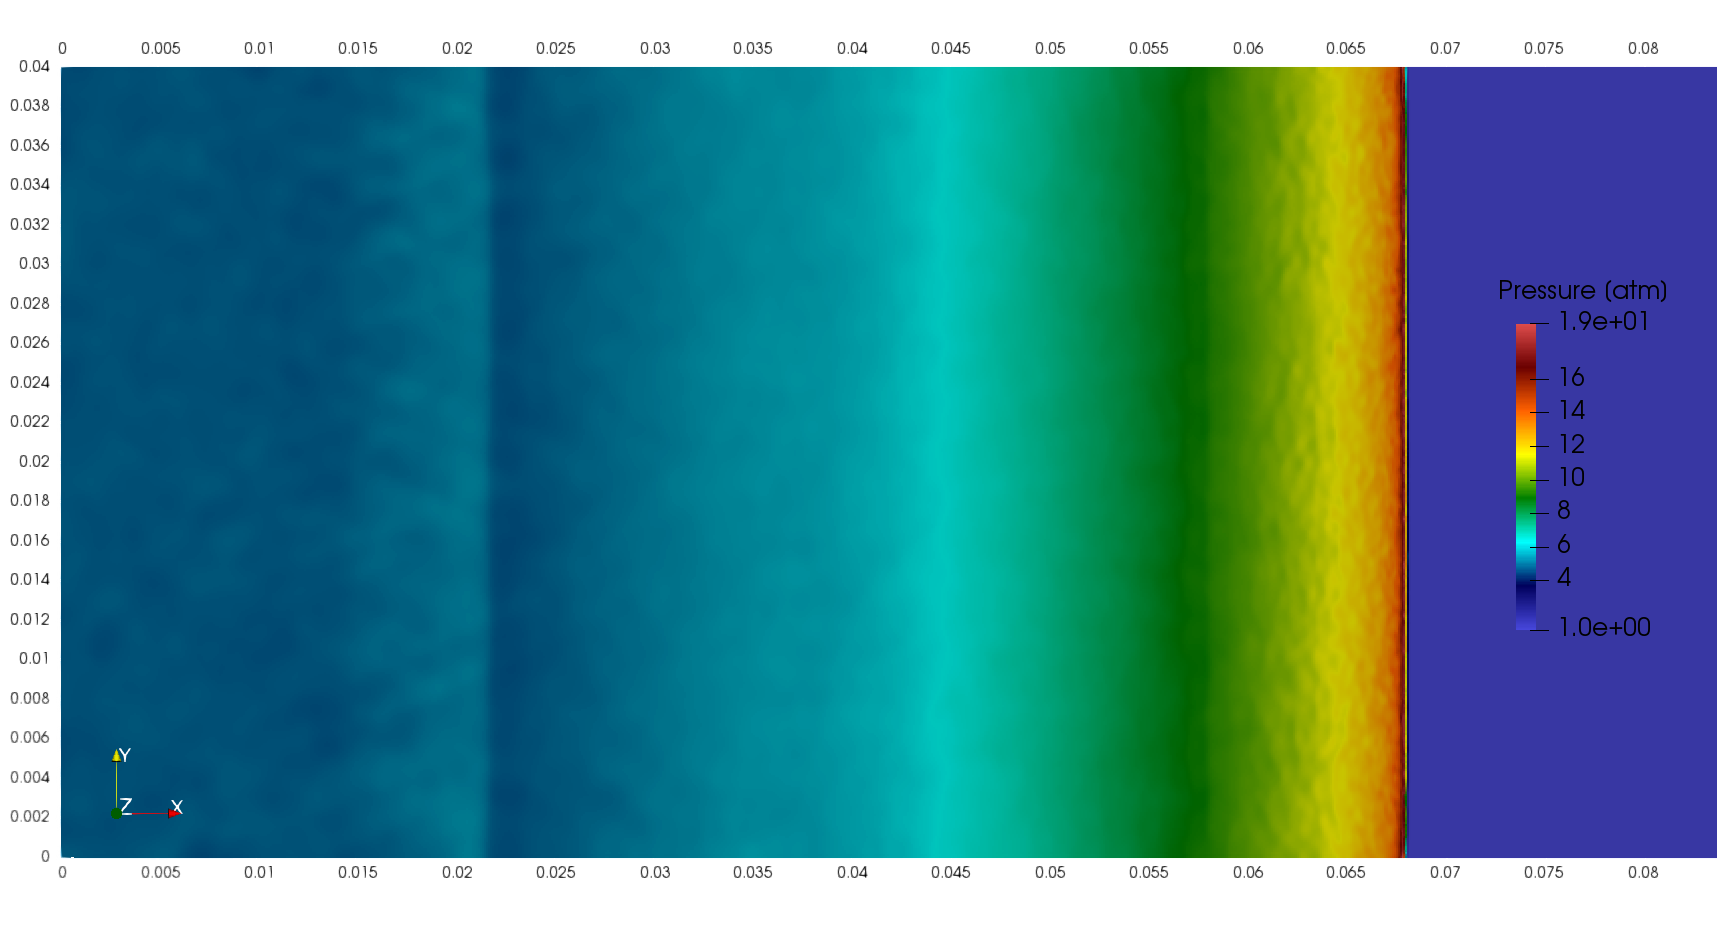
\includegraphics[width=0.8\linewidth]{../figs/Atest_refined/p.png}
%\caption{Pressure distribution in detonation tube for refined pre-exponential factor exponent sweep test, filtered from Figure \ref{fig:pjump} and refined from Figure \ref{fig:atestp}}
%\label{fig:atestrp}
\end{figure}
\end{frame}

\begin{frame}{Arrhenius Pre-exponential Factor Sweep, Refined: Temperature Distribution}
\begin{figure}
\centering
\includegraphics[width=0.8\linewidth]{../figs/Atest_refined/t.png}
%\caption{Temperature distribution in detonation tube for refined pre-exponential factor exponent sweep test, refined from Figure \ref{fig:atestt}}
%\label{fig:atestrt}
\end{figure}
\end{frame}

\begin{frame}{Arrhenius $A$ Variation: Temperature Distribution}
\begin{figure}
\centering
\includegraphics[width=0.8\linewidth]{../figs/Atest/t.png}
%\caption{Temperature distribution in detonation tube for pre-exponential factor exponent sweep test}
%\label{fig:atestt}
\end{figure}
\end{frame}

\begin{frame}{Arrhenius $A$ Variation: Velocity Distribution}
\begin{figure}
\centering
\includegraphics[width=0.8\linewidth]{../figs/Atest/u.png}
%\caption{Velocity distribution in detonation tube for pre-exponential factor exponent sweep test}
%\label{fig:atestu}
\end{figure}
\end{frame}

\subsection{Time Step Variation}

\begin{frame}{Time Step Variation: Temperature Distribution}
\begin{center}
\includegraphics[width=0.8\textwidth]{../figs/cfl_test/t.png}
\end{center}
\end{frame}

\begin{frame}{Time Step Variation: Velocity Distribution}
\begin{center}
\includegraphics[width=0.8\textwidth]{../figs/cfl_test/u.png}
\end{center}
\end{frame}

\subsection{Static Mesh Variation}

\begin{frame}{1D Static Mesh Variation: Temperature Distribution}
\begin{center}
\includegraphics[width=0.8\textwidth]{../figs/static1d/t.png}
\end{center}
\end{frame}

\begin{frame}{1D Static Mesh Variation: Velocity Distribution}
\begin{center}
\includegraphics[width=0.8\textwidth]{../figs/static1d/u.png}
\end{center}
\end{frame}

\begin{frame}{2D Static Mesh Variation: Temperature Distribution}
\begin{center}
\includegraphics[width=0.8\textwidth]{../figs/staticfigs/t.png}
\end{center}
\end{frame}

\begin{frame}{2D Static Mesh Variation: Velocity Distribution}
\begin{center}
\includegraphics[width=0.8\textwidth]{../figs/staticfigs/u.png}
\end{center}
\end{frame}

\subsection{AMR and Static Mesh Comparison}

\begin{frame}{AMR vs. Static: Temperature Distribution}
\begin{center}
\includegraphics[width=0.8\textwidth]{../figs/amrfigs/amrcompare/t.png}
\end{center}
\end{frame}

\begin{frame}{AMR vs. Static: Temperature Distribution (enlarged)}
\begin{center}
\includegraphics[width=0.8\textwidth]{../figs/amrfigs/amrcompare/te.png}
\end{center}
\end{frame}

\begin{frame}{AMR vs. Static: Velocity Distribution}
\begin{center}
\includegraphics[width=0.8\textwidth]{../figs/amrfigs/amrcompare/u.png}
\end{center}
\end{frame}

\begin{frame}{AMR vs. Static: Velocity Distribution (enlarged)}
\begin{center}
\includegraphics[width=0.8\textwidth]{../figs/amrfigs/amrcompare/ue.png}
\end{center}
\end{frame}


\subsection{AMR Refinement Level Variation}

\begin{frame}{AMR Refinement Level Variation: Temperature Distribution}
\begin{center}
\includegraphics[width=0.8\textwidth]{../figs/amrfigs/amr_refinelevels/t.png}
\end{center}
\end{frame}

\begin{frame}{AMR Refinement Level Variation: Temperature Distribution (enlarged)}
\begin{center}
\includegraphics[width=0.8\textwidth]{../figs/amrfigs/amr_refinelevels/te.png}
\end{center}
\end{frame}

\begin{frame}{AMR Refinement Level Variation: Velocity Distribution}
\begin{center}
\includegraphics[width=0.8\textwidth]{../figs/amrfigs/amr_refinelevels/u.png}
\end{center}
\end{frame}

\begin{frame}{AMR Refinement Level Variation: Velocity Distribution (enlarged)}
\begin{center}
\includegraphics[width=0.8\textwidth]{../figs/amrfigs/amr_refinelevels/ue.png}
\end{center}
\end{frame}

\subsection{AMR Buffer Layer Variation}

\begin{frame}{AMR Buffer Layer Variation: Temperature Distribution}
\begin{center}
\includegraphics[width=0.8\textwidth]{../figs/amrfigs/amr_bufflayers/t.png}
\end{center}
\end{frame}

\begin{frame}{AMR Buffer Layer Variation: Temperature Distribution (enlarged)}
\begin{center}
\includegraphics[width=0.8\textwidth]{../figs/amrfigs/amr_bufflayers/te.png}
\end{center}
\end{frame}

\begin{frame}{AMR Buffer Layer Variation: Velocity Distribution}
\begin{center}
\includegraphics[width=0.8\textwidth]{../figs/amrfigs/amr_bufflayers/u.png}
\end{center}
\end{frame}

\begin{frame}{AMR Buffer Layer Variation: Velocity Distribution (enlarged)}
\begin{center}
\includegraphics[width=0.8\textwidth]{../figs/amrfigs/amr_bufflayers/ue.png}
\end{center}
\end{frame}

\subsection{Refinement Range Variation}

\begin{frame}{AMR $|| \nabla (p)||$ Refine Range Variation: Temperature Distribution}
\begin{center}
\includegraphics[width=0.8\textwidth]{../figs/amrfigs/amr_refinebounds/t.png}
\end{center}
\end{frame}

\begin{frame}{AMR $|| \nabla (p)||$ Refine Range Variation: Temperature Distribution (enlarged)}
\begin{center}
\includegraphics[width=0.8\textwidth]{../figs/amrfigs/amr_refinebounds/te.png}
\end{center}
\end{frame}

\begin{frame}{AMR $|| \nabla (p)||$ Refine Range Variation: Velocity Distribution}
\begin{center}
\includegraphics[width=0.8\textwidth]{../figs/amrfigs/amr_refinebounds/u.png}
\end{center}
\end{frame}

\begin{frame}{AMR $|| \nabla (p)||$ Refine Range Variation: Velocity Distribution (enlarged)}
\begin{center}
\includegraphics[width=0.8\textwidth]{../figs/amrfigs/amr_refinebounds/ue.png}
\end{center}
\end{frame}

\begin{frame}{Previous Work}
\begin{itemize}
\item Towery \textit{et. al.} \cite{towery1} examined PDEs and RDEs with static grids with inviscid Euler equations using an in-house Fortran parallelized code, also focusing on turbulence modeling 
\item Marcantoni \textit{et. al.} \cite{marcantoni} developed \texttt{rhoReactingRfFoam}, a non-AMR OpenFOAM solver for detonations 
\item Berger and Jameson \cite{berger1985} used and developed adaptive mesh refinement routines to solve the Euler equations 
\item Deiterding \cite{deiterding} used the Berger and Colella \cite{berger1989} AMR routines to simulate detonations with the Euler equations, developing and implementing parallelization and distributed computing 
\end{itemize}
\end{frame}

\begin{frame}{Previous Work (ii)}
\begin{itemize}
\item Yi \textit{et. al.} \cite{yi} explored numerical simulations of RDEs in three dimensions, exploring overall flow-field and comparing to one- and two-dimensional simulations 
\item Schwer and Kailasanath \cite{schwer1} examined effects of different hydrocarbon fuels in RDEs as well as numerical methods for simulating them 
\item Li \textit{et. al.} \cite{li} used the Berger-Oliger AMR routines \cite{berger1984} and simulated detonations, noting the presence of cellular detonation structure 
\item Kim and Kim \cite{kim} simulated confined detonations in OpenFOAM with seven-step chemistry and compared to experimental results 
\end{itemize}
\end{frame}
